% This file was created by tikzplotlib v0.9.8.
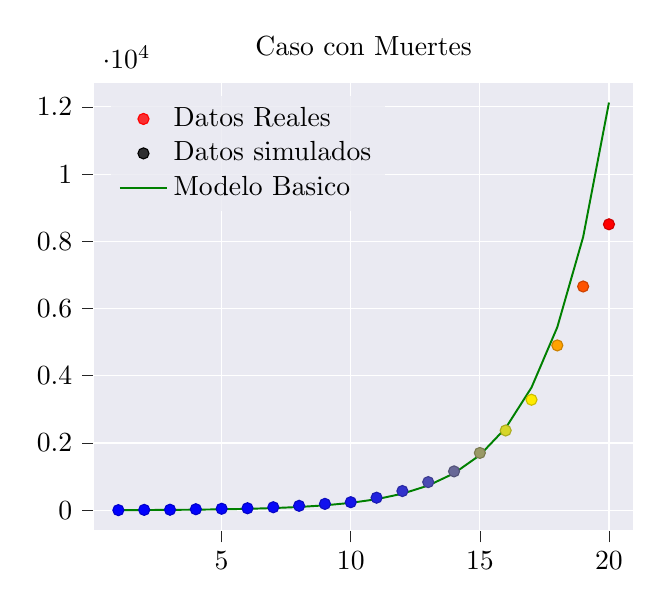
\begin{tikzpicture}

\definecolor{color0}{rgb}{0.917647058823529,0.917647058823529,0.949019607843137}

\begin{axis}[
axis background/.style={fill=color0},
axis line style={white},
legend cell align={left},
legend style={
  fill opacity=0.8,
  draw opacity=1,
  text opacity=1,
  at={(0.03,0.97)},
  anchor=north west,
  draw=none,
  fill=color0
},
tick align=outside,
tick pos=left,
title={Caso con Muertes},
x grid style={white},
xmajorgrids,
xmin=0.0499999999999999, xmax=20.95,
xtick style={color=white!15!black},
y grid style={white},
ymajorgrids,
ymin=-604.300586954471, ymax=12734.3123260439,
ytick style={color=white!15!black}
]
\addplot [draw=red, fill=red, mark=*, only marks, scatter]
table{%
x  y
1 2
2 10
3 14
4 29
5 43
6 58
7 88
8 130
9 188
10 238
11 372
12 570
13 836
14 1155
15 1704
};
\addlegendentry{Datos Reales}
\addplot [draw=black, fill=black, mark=*, only marks, scatter]
table{%
x  y
16 2372
17 3286
18 4903
19 6656
20 8506
};
\addlegendentry{Datos simulados}
\addplot [line width=0.7pt, green!50!black]
table {%
1 2
2 4.98382091522217
3 9.43541526794434
4 16.0767936706543
5 25.9851379394531
6 40.7674942016602
7 62.8214378356934
8 95.7239303588867
9 144.811462402344
10 218.045562744141
11 327.304046630859
12 490.307373046875
13 733.492553710938
14 1096.30041503906
15 1637.57141113281
16 2445.08569335938
17 3649.79541015625
18 5447.0478515625
19 8128.24072265625
20 12128.01171875
};
\addlegendentry{Modelo Basico}
\end{axis}

\end{tikzpicture}
